%************************************************
\chapter{Domain Name Service and Service Discovery}\label{ch:dns}
%************************************************
\textit{Topic 5: Write a brief introduction to Domain Name Service and Service Discovery and use these descriptions to put perspective on your report. The perspectives should include:
- How may Domain Name Services be beneficial in cluster and cloud computing?
- How may Service Discovery be beneficial in cluster and cloud computing?}
\section{DNS}
The Domain Name Service (DNS) is a service that allows humans readable language converting to IP address. In other word DNS allows to type names into the Web browser like www.youtube.com and automatically find that address on the Internet (IP), instead of type the IP-address of the web site.

The DNS organizes its servers into a hierarchy figure \ref{fig:DNShierarchy} shows the hierarchy. For the Internet, so-called root name servers reside at the top of the DNS hierarchy. The root servers are responsible for holding information about all the top level domains, it is the starting point for every name lookup operation. Top level domains are divided into two groups:

\begin{itemize}
\item \textbf{Generic Top Level Domains (gTLD) .com, .edu, .net, .org, .mil etc.}
\item \textbf{ Country Code Top Level Domain (ccTLD) e.g. .us, .ca, .tv , .uk etc.}
\end{itemize}
Each ccTLD identifies a particular country and is two letters long.   

\textbf{At the domain level or user DNS you have the resource you are looking for.??
}

\begin{figure}[bth]
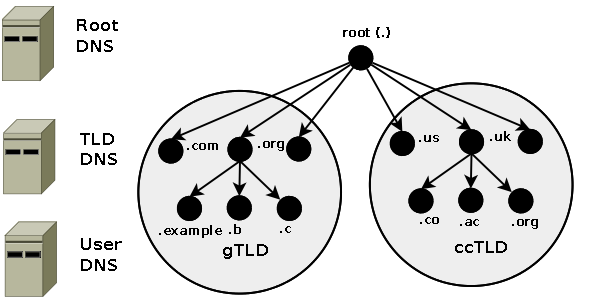
\includegraphics[width=1\linewidth]{gfx/DNShierarchy}
\caption[routingtable]{Routing table for Pastry} \label{fig:DNShierarchy}
\end{figure}
\\
\textbf{Recursive Query Vs Iterative Query in DNS}

A recursive query is a kind of query, in which the DNS server, who received the query, will do the entire job fetching the answer, and giving it back to client. If DNS server is not able to resolve the requested query then it forwards the query to another DNS server until it gets an answer or the query fails.
In an iterative query, the name server, will not go and fetch the complete answer for the query. If the queried DNS server doesn't have an exact match for the queried name, the best possible information it can return is a referral, which might have the answer. The DNS client can then query the DNS server for which it obtained a referral.
\\\\
\textbf{Cached queries}

DNS caching allows any DNS server or client to locally store the DNS records and re-use them in the future. The Ip and domain is stored in local cache called stub-resolver for a period. By that, the overall network usage is reduced and thereby higher efficiency is achieved. The number of packets sent out also gets reduced and thereby a lower latency. 
\\\\
\textbf{How may Domain Name Services be beneficial in cluster and cloud computing?}


By having redundant Domain Name Services, the concept of single point of failure is avoided, in the case of failure of a single or multiple DNS services. Hence by having redundant DNS in cloud computing it becomes fault tolerant.  
   

To create additional resilience each root-server typically has multiple instances (copies) spread throughout the world. Each instance has the same IP address but data is sent to the closest instance using a process called anycasting.

\section{Service Discovery}
Service discovery protocols (SDP) are network protocols which allows automatic finding available services, on the same network. The service discovery requires a common language to allow software agents to make use of each other's services without the need for user intervention.


\textbf{Service Discovery in a Microservices Architecture}

The issue not having the service discovery could for instance be if you have some code to invoke a service that has a REST API. To make a request on a specific service you need to know it's IP address and port number. In a cloud-based microservices application the problem occurs while      



\textbf{How may Service Discovery be beneficial in cluster and cloud computing?}  
